\documentclass[9pt]{article}

\usepackage{amsmath}
\usepackage{tcolorbox}
% `parskip` removes indentation for all paragraphs: http://tex.stackexchange.com/a/55016
\usepackage{parskip}
% Allows us to color rows / cols of a table.
% See https://texblog.org/2011/04/19/highlight-table-rowscolumns-with-color/
\usepackage{color, colortbl}

\usepackage{hyperref}
\graphicspath{{images/ps6/}}

\leftmargin=0.25in
\oddsidemargin=0.25in
\textwidth=6.0in
\topmargin=-0.25in
\textheight=9.25in

\definecolor{Gray}{gray}{0.9}

\begin{document}

\begin{center}
  \large\textbf{MIT 18.01 Problem Set 6 Unofficial Solutions}
\end{center}

\begin{tcolorbox}
  \textbf{Q1)} Do 7.4/12 and 13.
\end{tcolorbox}

\textbf{Skipped.} We do not have the textbook.


\begin{tcolorbox}
  \textbf{Q2)} The voltage $V$ of the house current is given by\\
  \begin{center}
    $V(t) = Csin(120\pi t)$
  \end{center}
  where $t$ is time, in seconds and $C$ is a constant amplitude. The square root of the average value of $V^2$ over one period of $V(t)$ (or cycle) is called the \emph{root-mean-square} voltage, abbreviated RMS. This is what the voltage meter on a house records. For house current, find the RMS in terms of the constant $C$. (The peak voltage delivered to the house is $\pm C$. The units of $V^2$ are square volts; when we take the square root again after averaging, the units become volts again.)
\end{tcolorbox}

Every cycle of the $sin$ function corresponds to $2 \pi$. This happens every $t = \frac{2 \pi}{120 \pi} = \frac{1}{60}$ seconds.

Since $V(t) = Csin(120\pi t)$, $V^2(t) = C^2 sin^2(120\pi t)$. The average value of $V^2$ over 1 cycle of $V(t)$ is:

\begin{align*}
  \frac{1}{\frac{1}{60} - 0} \int_0^{\frac{1}{60}} C^2 sin^2(120\pi t) dt &= 60C^2 \int_0^{\frac{1}{60}} sin^2(120\pi t) dt \\
  &= 60C^2(\frac{1}{2}t - \frac{1}{240\pi} sin(120\pi t) cos(120\pi t)) \bigg]_0^{1/60} \\
  &= 60C^2(\frac{1}{2} \cdot \frac{1}{60} - \frac{1}{240\pi} sin(2\pi) cos(2\pi) - (\frac{1}{2} \cdot 0 - \frac{1}{240\pi} sin(0) cos(0))) \\
  &= 60C^2 \cdot \frac{1}{120} \\
  &= \frac{C^2}{2}
\end{align*}

Then RMS $= \sqrt{\frac{C^2}{2}} = \frac{C}{\sqrt{2}} = \frac{\sqrt{2}C}{2}$


\begin{tcolorbox}
  \textbf{Q3a)} What is the probability that $x^2 < y$ if $(x, y)$ is chosen from the unit square $0 \leq x \leq 1$, $0 \leq y \leq 1$ with probability equal to the area.
\end{tcolorbox}

\begin{center}
  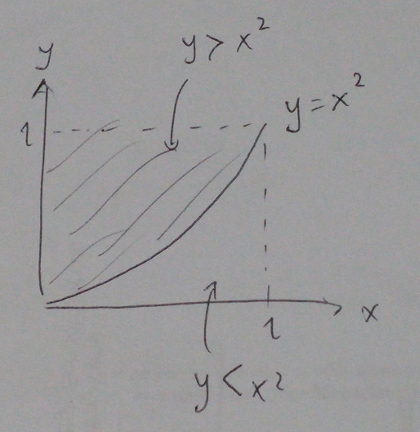
\includegraphics[scale=0.4]{q3a.jpg}
\end{center}

\begin{align*}
  P(x^2 < y) &= \frac{\int_0^1 1 dx - \int_0^1 x^2 dx}{\int_0^1 1 dx} \\
  &= \frac{x \bigg]_0^1 - \frac{x^3}{3}\bigg]_0^1}{x \bigg]_0^1} \\
  &= \frac{1 - \frac{1}{3}}{1} \\
  &= \frac{2}{3}
\end{align*}


\begin{tcolorbox}
  \textbf{Q3b)} What is the probability that $x^2 < y$ if $(x, y)$ is chosen from the square $0 \leq x \leq 2$, $0 \leq y \leq 2$ with probability \textbf{proportional} to the area. (Probability = Part/Whole).
\end{tcolorbox}

\begin{center}
  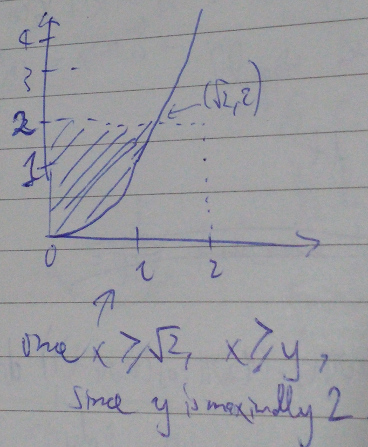
\includegraphics[scale=0.5]{q3b.jpg}
\end{center}

For the line $y = x^2$ $y = 2$, $x = \sqrt{2}$. Once $x \ge \sqrt{2}$, $y > 2$. Hence $x \leq \sqrt{2}$.

\begin{align*}
  P(x^2 < y) &= \frac{\int_0^2 2 dx - \int_0^{\sqrt{2}} x^2 dx - \int_{\sqrt{2}}^2 2 dx}{\int_0^2 2 dx} \\
  &= \frac{2x \bigg]_0^2 - \frac{x^3}{3} \bigg]_0^{\sqrt{2}} - 2x \bigg]_{\sqrt{2}}^2}{2x \bigg]_0^2} \\
  &= \frac{4 - \frac{(\sqrt{2})^3}{3} - (4 - 2\sqrt{2})}{4} \\
  &= \frac{4 - \frac{2\sqrt{2}}{3} - 4 + 2\sqrt{2}}{4} \\
  &= \frac{2\sqrt{2} - \frac{2\sqrt{2}}{3}}{4} \\
  &= \frac{\frac{6 \sqrt{2} - 2\sqrt{2}}{3}}{4} \\
  &= \frac{\frac{4 \sqrt{2}}{3}}{4} \\
  &= \frac{\sqrt{2}}{3}
\end{align*}


\begin{tcolorbox}
  \textbf{Q3c)} Evaluate \\
  \begin{center}
    $W = \int_0^{\infty} e^{-at} dt = \lim\limits_{N \rightarrow \infty} \int_0^N e^{-at} dt$
  \end{center}
  This is known as an improper integral because it represents the area of an unbounded region. We are using the letter $W$ to signify "whole". \\
  The probability that a radioactive particle will decay some time in the interval $0 \leq t \leq T$ is \\
  \begin{center}
    $P([0, T]) = \frac{\text{PART}}{\text{WHOLE}} = \frac{1}{W} \int_0^T e^{-at} dt$
  \end{center}
  \begin{center}
  \end{center}
  Note that $P([0, \infty)) = 1 = 100\%$
\end{tcolorbox}

\begin{align*}
  \int_0^{\infty} e^{-at} dt &= -\frac{1}{a} e^{-at} \bigg]_0^{\infty} \\
  &= -\frac{1}{a} (e^{-a \cdot \infty} - e^{-a \cdot 0}) \\
  &= -\frac{1}{a} (\frac{1}{e^{a \cdot \infty}} - \frac{1}{e^{a \cdot 0}}) \\
  &= -\frac{1}{a} (0 - \frac{1}{e^0}) \\
  &= -\frac{1}{a} (-1) \\
  &= \frac{1}{a}
\end{align*}


\begin{tcolorbox}
  \textbf{Q3d)} The half-life is the time $T$ for which $P([0, T]) = 1/2$. Find the value of $a$ and $W$ for which the half-life is $T = 1$. Suppose that a radioactive particle has a half-life of 1 second. What is the probability that it survives to time $t = 1$, but decays some time during the interval $1 \leq t \leq 2$? (Give an integral formula, and use a calculator to get an approximate numerical answer.)
\end{tcolorbox}

We saw in part (c) that $W = \frac{1}{a}$. We want to find $a$ and $W$ such that $P([0, 1]) = \frac{1}{2}$

\begin{align*}
  P([0, 1]) &= \frac{\int_0^1 e^{-at} dt}{W} \\
  &= a \int_0^1 e^{-at} dt \\
  &= a(-\frac{1}{a} e^{-at} \bigg]_0^1) \\
  &= a \cdot (-\frac{1}{a}) e^{-at} \bigg]_0^1 \\
  &= -1(e^{-a} - e^0) \\
  &= -1(\frac{1}{e^a} - 1) \\
  &= 1 - \frac{1}{e^a} \\
  &= \frac{1}{2}
\end{align*}

So $1 - \frac{1}{e^a} = \frac{1}{2}$. Then $\frac{1}{2} = \frac{1}{e^a}$ and $e^a = 2$ so $a = ln(2)$ and $W = \frac{1}{a} = \frac{1}{ln(2)}$

From $0 \leq t \leq 1$, the particle decays with probability $\frac{1}{2}$ and survives with probability $\frac{1}{2}$. These 2 cases are mutually exclusivge and from $1 \leq t \leq 2$, the particle decays with probability $\frac{1}{W} \int_1^2 e^{-at} dt$ regardless of what happens from $0 \leq t \leq 1$.

Hence probability of particule surviving to $t = 1$ and decaying some time in $1 \leq t \leq 2$ is

\begin{align*}
  \frac{1}{2} \cdot \frac{1}{W} \int_1^2 e^{-at} dt &= \frac{1}{2} * a(-\frac{1}{a} e^{-at} \bigg]_1^2) \\
  &= -\frac{1}{2} (e^{-at} \bigg]_1^2) \\
  &= -\frac{1}{2} (e^{-2a} - e^{-a}) \\
  &= \frac{1}{2} e^{-a} - \frac{1}{2} e^{-2a} \\
  &= \frac{1}{2} e^{-ln(2)} - \frac{1}{2} e^{-2ln(2)} \\
  &= \frac{1}{2} e^{ln(2^{-1})} - \frac{1}{2} e^{ln(2^{-2})} \\
  &= \frac{1}{2} e^{ln(\frac{1}{2})} - \frac{1}{2} e^{ln(\frac{1}{4})} \\
  &= \frac{1}{2} \cdot \frac{1}{2} - \frac{1}{2} \cdot \frac{1}{4} \\
  &= \frac{1}{4} - \frac{1}{8} \\
  &= \frac{1}{8}
\end{align*}


\begin{tcolorbox}
  \textbf{Q4)} The basis for Simson's rule is the following formula. Let $x_1$ be the midpoint of the interval $[x_0, x_2]$, and denote its length by $2h$. Consider any three points $(x_0, y_0)$, $(x_1, y_1)$, $(x_2, y_2)$. There is a unique quadratic function (parabola) \\
  \begin{center}
    $y = Ax^2 + Bx + C$
  \end{center}
  \begin{center}
  \end{center}
  whose graph passes through the three points. Simpson's rule says that the area under the parabola above $[x_0, x_2]$ is
  \begin{center}
    $\frac{h}{3}(y_0 + 4y_1 + y_2)$
  \end{center}
  \begin{center}
  \end{center}
  This problem is devoted to proving this formula. It is significant because it illustrates how calculations can be simplified by using symmetry, and by looking ahead to see what you need.\\
  \\
  Since the area will be the same if the parabola is translated to the left or right, we may assume that $x_0 = -h$, $x_1 = 0$, and $x_2 = h$. Then in terms of the rest of the data (i.e., $h$ and the $y_i$) \\
  \\
  make a sketch and determine $C$;\\
  \\
  show, by integrating, that to find the area we need only determine $A$ (or better, $2Ah^2$);\\
  \\
  determine $2Ah^2$ using the data;\\
  \\
  put the results together to establish the formula for area.
\end{tcolorbox}

Since we are assuming that $x_1 = 0$, the easiest way to get $C$ is to substitute $x = x_1 = 0$ and $y = y_1$ into $y = Ax^2 + Bx + C$. From that, we get $y_1 = A(0)^2 + B(0) + C$ or $y_1 = C$.

Again, substituting $(x_2, y_2)$ into $y = Ax^2 + Bx + C$, we get $f(x_2) = f(h) = A(h^2) + B(h) + C = Ah^2 + Bh + y_1 = y_2$. Then $Bh = -Ah^2 - y_1 + y_2$ and $B = -Ah - \frac{y_1}{h} - \frac{y_2}{h}$ assuming $h \neq 0$.

\begin{align*}
  \int_{-h}^h Ax^2 + Bx + C dx &= \int_{-h}^h Ax^2 + (-Ah - \frac{y_1}{h} + \frac{y_2}{h})x + y_1 dx \\
  &= \bigg[ \frac{Ax^3}{3} - \frac{Ahx^2}{2} - \frac{y_1x^2}{2h} + \frac{y_2x^2}{2h} + y_1x \bigg]_{-h}^h \\
  &= \frac{Ah^3}{3} - \frac{Ahh^2}{2} - \frac{y_1h^2}{2h} + \frac{y_2h^2}{2h} + y_1h - (\frac{A(-h)^3}{3} - \frac{Ah(-h)^2}{2} - \frac{y_1(-h)^2}{2h} + \frac{y_2(-h)^2}{2h} + y_1(-h)) \\
  &= \frac{Ah^3}{3} - \frac{Ah^3}{2} - \frac{y_1h}{2} + \frac{y_2h}{2} + y_1h - (-\frac{Ah^3}{3} - \frac{Ah^3}{2} - \frac{y_1h}{2} + \frac{y_2h}{2} - y_1h) \\
  &= \frac{2Ah^3}{3} + 2y_1h \\
  &= \frac{h}{3}(2Ah^2 + 6y_1)
\end{align*}

If we know $x_0$ and $x_2$, then we will know $h$. We will also know $x_1$ and hence $y_1$. Then we only need to determine $A$ to find the area.

Now we will determine $2Ah^2$ from the data. Earlier, we have that $y_2 = Ah^2 + Bh + y_1$. From this, we get $Ah^2 = y_2 - Bh - y_1$.

If we substitute $(x_0 = -h, y_0)$ into $y = Ax^2 + Bx + C$, we get $y_0 = A(-h)^2 + B(-h) + C = Ah^2 - Bh + C$ and $Ah^2 = y_0 + Bh - C$ and since $C = y_1$, this is $Ah^2 = y_0 + Bh - y_1$.

Now we have

\begin{align*}
  Ah^2 &= y_2 - Bh - y_1 \\
  Ah^2 &= y_0 + Bh - y_1
\end{align*}

Adding them together gives us $2Ah^2 = y_2 - Bh - y_1 + y_0 + Bh - y_1 = y_0 - 2y_1 + y_2$. Then $2Ah^2 + 6y_1 = y_0 - 2y_1 + y_2 + 6y_1 = y_0 + 4y_1 + y_2$.

Then

\begin{align*}
  \int_{-h}^h Ax^2 + Bx + C dx &= \frac{h}{3}(2Ah^2 + 6y_1) \\
  &= \frac{h}{3}(y_0 + 4y_1 + y_2)
\end{align*}

which is exactly what we want.


\begin{tcolorbox}
  \textbf{Q5)} Use a calculator to make a table of values of the integrand and find approximations to the Fresnel integral $\int_0^a cos(t^2) dt$ for $a = \sqrt{\pi / 2}$, using Simpson's rule with four and eight intervals. (The exact answer to five decimal places is $1.22505$. Record your approximations to six decimal places to compare.)
\end{tcolorbox}

With 4 intervals, each interval is of size $\frac{1}{4} \sqrt{\frac{\pi}{2}}$.

\begin{center}
  \begin{tabular}{|c|c|}
    \hline
    \rowcolor{Gray}
    $x$ & $cos(x^2)$ \\ \hline
    $0$ & $cos(0^2) = 1$ \\ \hline
    $\frac{1}{4} \sqrt{\frac{\pi}{2}}$ & $cos(\frac{1}{16} \cdot \frac{\pi}{2}) = cos(\frac{\pi}{32})$ \\ \hline
    $\frac{1}{2} \sqrt{\frac{\pi}{2}}$ & $cos(\frac{1}{4} \cdot \frac{\pi}{2}) = cos(\frac{\pi}{8})$ \\ \hline
    $\frac{3}{4} \sqrt{\frac{\pi}{2}}$ & $cos(\frac{9}{16} \cdot \frac{\pi}{2}) = cos(\frac{9\pi}{32})$ \\ \hline
    $\sqrt{\frac{\pi}{2}}$ & $cos(\frac{\pi}{2}) = 0$ \\ \hline
  \end{tabular}
\end{center}

\begin{align*}
  \int_0^a cos(t^2) dt &= \frac{\frac{1}{4} \sqrt{\frac{\pi}{2}}}{3} (cos(0^2 ) + 4cos(\frac{\pi}{32}) + 2cos(\frac{\pi}{8}) + 4cos(\frac{9\pi}{32}) + cos(\frac{\pi}{2})) \\
  &\approx 0.978219
\end{align*}

With 8 intervals, each interval is of size $\frac{1}{8} \sqrt{\frac{\pi}{2}}$

\begin{center}
  \begin{tabular}{|c|c|}
    \hline
    \rowcolor{Gray}
    $x$ & $cos(x^2)$ \\ \hline
    $0$ & $cos(0^2) = 1$ \\ \hline
    $\frac{1}{8} \sqrt{\frac{\pi}{2}}$ & $cos(\frac{1}{64} \cdot \frac{\pi}{2}) = cos(\frac{\pi}{128})$ \\ \hline
    $\frac{2}{8} \sqrt{\frac{\pi}{2}}$ & $cos(\frac{4}{64} \cdot \frac{\pi}{2}) = cos(\frac{\pi}{32})$ \\ \hline
    $\frac{3}{8} \sqrt{\frac{\pi}{2}}$ & $cos(\frac{9}{64} \cdot \frac{\pi}{2}) = cos(\frac{9\pi}{128})$ \\ \hline
    $\frac{4}{8} \sqrt{\frac{\pi}{2}}$ & $cos(\frac{16}{64} \cdot \frac{\pi}{2}) = cos(\frac{\pi}{8})$ \\ \hline
    $\frac{5}{8} \sqrt{\frac{\pi}{2}}$ & $cos(\frac{25}{64} \cdot \frac{\pi}{2}) = cos(\frac{25\pi}{128})$ \\ \hline
    $\frac{6}{8} \sqrt{\frac{\pi}{2}}$ & $cos(\frac{36}{64} \cdot \frac{\pi}{2}) = cos(\frac{9\pi}{32})$ \\ \hline
    $\frac{7}{8} \sqrt{\frac{\pi}{2}}$ & $cos(\frac{49}{64} \cdot \frac{\pi}{2}) = cos(\frac{49\pi}{128})$ \\ \hline
    $\sqrt{\frac{\pi}{2}}$ & $cos(\frac{\pi}{2}) = 0$ \\ \hline
  \end{tabular}
\end{center}

\begin{align*}
  \int_0^a cos(t^2) dt &= \frac{\frac{1}{8} \sqrt{\frac{\pi}{2}}}{3} (cos(0^2) + 4cos(\frac{\pi}{128}) + 2cos(\frac{\pi}{32}) + 4cos(\frac{9\pi}{128}) + 2cos(\frac{\pi}{8}) + 4cos(\frac{25\pi}{128}) + 2cos(\frac{9\pi}{32}) \\
  & \ \ \ + 4cos(\frac{49\pi}{128}) + cos(\frac{\pi}{2})) \\
  &\approx 0.977503
\end{align*}

\end{document}
